% This is samplepaper.tex, a sample chapter demonstrating the
% LLNCS macro package for Springer Computer Science proceedings;
% Version 2.21 of 2022/01/12
%

\documentclass[runningheads]{llncs}
%
\usepackage[T1]{fontenc}
\usepackage{enumitem}
% T1 fonts will be used to generate the final print and online PDFs,
% so please use T1 fonts in your manuscript whenever possible.
% Other font encondings may result in incorrect characters.
%

\usepackage{graphicx}
\usepackage{float}

% Used for displaying a sample figure. If possible, figure files should
% be included in EPS format.
%
% If you use the hyperref package, please uncomment the following two lines
% to display URLs in blue roman font according to Springer's eBook style:
%\usepackage{color}
\usepackage{multirow}
%\renewcommand\UrlFont{\color{blue}\rmfamily}
%\urlstyle{rm}
%
\begin{document}
%
\title{Hide-and-Seek: A Multi-Agent Reinforcement Learning Simulator}
%
%\titlerunning{Abbreviated paper title}
% If the paper title is too long for the running head, you can set
% an abbreviated paper title here
%
\author{Jakub Szafrański\inst{1}\orcidID{0009-0006-0548-3461}}
%
\authorrunning{Szafrański J.}
% First names are abbreviated in the running head.
% If there are more than two authors, 'et al.' is used.
%
\institute{Wrocław University of Science and Technology, Faculty of Information and Communication Technology,\\
Wrocław, Poland\\
\email{266498@student.pwr.edu.pl}}
%
\maketitle              % typeset the header of the contribution
%
\begin{abstract}
This paper presents a hide-and-seek simulator developed to investigate learning processes in multi-agent systems using tabular reinforcement learning algorithms. The simulator offers a configurable 2D environment with real-time visualization, data logging, and adjustable parameters, including state representations, reward schemes, game rules, and the selection of learning algorithms along with their parameters. It facilitates the analysis of how these factors influence the learning capabilities of the agent. The research examines their impact by comparing performance metrics, such as success rate and average cumulative reward, across configurations. Experimental results show that Monte Carlo underperformed relative to Q-learning and Sarsa. Relative state representations boost both success rates and rewards over full representations. Continuous rewards consistently achieve higher success rates, while terminal ones, though less reliable, can yield higher average returns. The simulator serves as a versatile tool for both educational and research purposes into multi-agent reinforcement learning.

\keywords{Reinforcement Learning \and Multi-Agent Systems \and Hide-and-Seek}
\end{abstract}


\section{Introduction}
Reinforcement learning (RL) involves agents learning to map situations to actions to maximize a numerical reward through trial-and-error exploration, where actions influence immediate and future outcomes~\cite{ref_rlbook}. In multi-agent systems~\cite{ref_multiagent}, several agents coexist and interact within a shared environment, meaning an agent’s behavior is shaped not only by the environment but also by the actions of others. This dynamic is exemplified in a hide-and-seek game, where a seeker and a hider adapt their strategies based on mutual interactions. This work introduces a configurable simulator designed to study such learning processes in a multi-agent hide-and-seek scenario, analyzing their impact through evaluation of success rates and cumulative rewards. Reinforcement learning has been widely applied to various game-based environments, proving its effectiveness as a framework for developing intelligent game-playing agents. This approach spans simple games, such as Snake~\cite{ref_snake} or Pac-Man~\cite{ref_pacman}, to complex environments such as Minecraft~\cite{ref_minecraft} or Gran Turismo~\cite{ref_granturismo}. Multi-agent hide-and-seek using RL has been explored by researchers investigating how agents optimize seeking and hiding behaviors through tabular~\cite{ref_hideandseek} and policy gradient~\cite{ref_hs2} methods, demonstrating effectiveness in competitive multi-agent environments.


\section{Simulation Environment}

The hide-and-seek simulator operates on a static, 2D $N \times M$ grid populated with obstacles, as shown in Figure \ref{env_visualization}. The seeker attempts to locate the hider within a limited field of view, while the hider aims to avoid detection. The game ends when the seeker finds the hider or after a configurable maximum number of moves is reached, at which point the hider is declared the winner if undetected. In each turn, both agents select one of the five available actions: moving up, down, left, right, or staying in place. 

\begin{figure}[H]
\centering
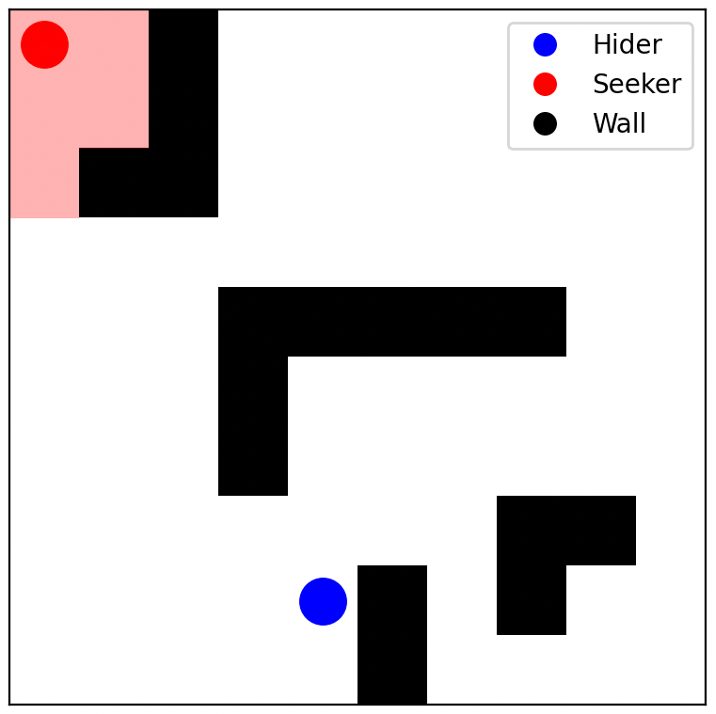
\includegraphics[width=0.6\textwidth]{env.png}  % Adjust the width to make the figure smaller
\caption{Visualization of the hide-and-seek environment.}
\label{env_visualization}
\end{figure}

The simulator, implemented in Python, offers a versatile platform supporting:
\begin{itemize}
    \item Configuration of rules (e.g., seeker’s range of view, maximum move limit) and grid layout.
    \item Various state definitions:
        \begin{itemize}[label=--]
            \item Relative position: The agent is aware of its own coordinates $(x, y)$ and the relative direction of its opponent (e.g., left, right, below, above).
            \item Full positional knowledge: The agent has access to its own coordinates $(x, y)$ and the exact coordinates $(x, y)$ of its opponent.
        \end{itemize}
    \item Reward schemes:
        \begin{itemize}[label=--]
            \item Continuous: Seeker receives -1 per move, hider receives +1 per move, winner receives +30, and loser receives -30.
            \item Terminal: Winner receives +30, and loser receives -30 at the end of the game.
        \end{itemize}
    \item Reinforcement learning algorithms: Q-learning, Sarsa, and Monte Carlo Control~\cite{ref_rlbook}.
    \item Action selection strategies: $\varepsilon$-greedy~\cite{ref_rlbook} with fixed or linearly decaying $\varepsilon$.
    \item Data logging: Each episode’s data—length, agents’ actions and returns, and the winner—is recorded in a JSON file.
    \item Real-time visualization. \end{itemize}

The hide-and-seek simulator is open-source and accessible at  the GitHub repository \url{https://github.com/jakub-szafranski/marl-hide-and-seek}.

\section{Research Scope}
This study explores the effects of simulator parameters on agent learning in the hide-and-seek environment, measuring learning effectiveness through success rate and average cumulative reward, reflecting agent performance and policy quality. The investigation focuses on:
\begin{itemize}
    \item Comparing algorithms: Q-learning, Sarsa, and Monte Carlo Control.
    \item Assessing state definitions: relative position, and full positional knowledge.
    \item Evaluating reward schemes: continuous and terminal.
\end{itemize}
Each configuration undergoes a training phase of 5,000 episodes, based on observed stabilization in preliminary runs. Performance is then evaluated over 1,000 episodes with fixed policies, and the results are averaged to mitigate randomness. This process is repeated 50 times for each configuration to ensure statistical significance of the evaluation. The initial positions of the seeker and hider are randomized, while other parameters remain constant to isolate the effects of the investigated factors. In all configurations, only the seeker agent is learning, while the hider uses a fixed, pre-trained policy. Statistical tests were conducted using the Mann-Whitney U test at a significance level of 0.05. To account for multiple comparisons, a Bonferroni correction was applied.

\section{Results}
The experiments revealed distinct patterns in agent learning behaviors across different configurations. Table~\ref{tab:results} summarizes the key performance metrics for seeker agent under various learning conditions.
\\

\begin{table}
\caption{Performance metrics for seeker agent across configurations (mean ± SD).}
\label{tab:results}
\begin{normalsize}
\begin{tabular}{|l|l|l|c|c|}
\hline
\textbf{Algorithm} & \textbf{State} & \textbf{Reward} & \textbf{Success Rate} & \textbf{Avg. Reward} \\
\hline
\multirow{4}{*}{Q-learning} 
 & Full & Terminal & 69.27\% ± 12.25\% & 19.27 ± 11.76 \\
 & Full & Continuous & 76.79\% ± 11.97\% & 10.94 ± 12.59 \\
 & Relative & Terminal & 86.12\% ± 7.54\% & 36.12 ± 7.28 \\
 & Relative & Continuous & 89.97\% ± 4.81\% & 25.51 ± 5.48 \\
\hline
\multirow{4}{*}{Sarsa} 
 & Full & Terminal & 72.23\% ± 10.46\% & 22.23 ± 9.67 \\
 & Full & Continuous & 80.09\% ± 11.65\% & 14.45 ± 12.25 \\
 & Relative & Terminal & 87.98\% ± 6.80\% & 37.98 ± 5.98 \\
 & Relative & Continuous & 91.93\% ± 5.90\% & 27.83 ± 6.52 \\
\hline
\multirow{4}{*}{Monte Carlo} 
 & Full & Terminal & 29.80\% ± 13.52\% & -20.20 ± 11.84 \\
 & Full & Continuous & 34.43\% ± 14.80\% & -34.36 ± 15.57 \\
 & Relative & Terminal & 19.20\% ± 13.14\% & -30.80 ± 12.36 \\
 & Relative & Continuous & 16.84\% ± 13.88\% & -52.64 ± 15.18 \\
\hline
\end{tabular}
\end{normalsize}
\end{table}



A primary observation is that the Monte Carlo method consistently underperformed across all configurations, exhibiting the lowest outcomes in both success rate and average reward. Statistical analysis was conducted using the Mann-Whitney U test at a significance level of 0.05, confirming that Monte Carlo’s success rates and average rewards were significantly lower than those of Q-learning and Sarsa across all configurations, highlighting its difficulty in achieving effective policy convergence.

The comparison of reward schemes reveals that continuous rewards consistently yield higher success rates than terminal rewards, suggesting that incremental feedback facilitates the agent’s ability to reach its objective. Mann-Whitney U test at a significance level of 0.05 confirmed that continuous rewards produced significantly higher success rates than terminal rewards across all algorithms and state representations. However, an intriguing pattern emerges: terminal rewards, despite lower success rates, produce higher average rewards. The Mann-Whitney U test further validated that terminal rewards resulted in significantly higher average rewards than continuous rewards, indicating that while the agent is less likely to succeed with terminal rewards, successful episodes are completed more efficiently.

Another notable finding is the superior performance of relative state representations over full state representations across most configurations. Statistical analysis using the Mann-Whitney U test at a significance level of 0.05 confirmed that relative state representations yielded significantly higher success rates and average rewards than full state representations for Q-learning and Sarsa. This may be attributed to the relative state representation requiring a Q-table four times smaller, which facilitates faster convergence. However, while relative states accelerate learning in the short term, full state representations could potentially outperform given sufficient training steps, as they encapsulate more comprehensive environmental information. 

Overall, Sarsa and Q-learning combined with relative state representations and continuous rewards achieved the highest success rates, while the combination of relative state representations and terminal rewards yielded the highest average rewards.


\section{Conclusion}
The hide-and-seek simulator was implemented to explore multi-agent reinforcement learning dynamics. The simulator provides a versatile platform for studying agent learning, combining high configurability with real-time visualization. It can be effectively used in educational settings to teach concepts of reinforcement learning, multi-agent systems, and algorithm optimization through hands-on experimentation. Conducted experiments validate its effectiveness, demonstrating the influence of algorithm selection and reward structure on learning performance. Future enhancements could extend the platform’s capabilities by incorporating deep reinforcement learning algorithms and introducing multiple seekers and hiders as team members, facilitating a fully dynamic environment and enabling the study of agent cooperation.



















\begin{credits}


\subsubsection{\discintname}
The author has no competing interests to declare that are
relevant to the content of this article.
\end{credits}










%
% ---- Bibliography ----
%
% BibTeX users should specify bibliography style 'splncs04'.
% References will then be sorted and formatted in the correct style.
%
% \bibliographystyle{splncs04}
% \bibliography{mybibliography}
%
\begin{thebibliography}{8}

\bibitem{ref_rlbook}
Sutton, R.S., Barto, A.G.: Reinforcement Learning: An Introduction. 2nd edn. The MIT Press, Cambridge, Massachusetts (2018).

\bibitem{ref_multiagent}
G. Weiss, Ed., Multiagent Systems: A Modern Approach to Distributed Artificial Intelligence. Cambridge, MA: MIT Press, 1999.

\bibitem{ref_snake}
Ray, D., Ghosh, A., Ojha, M., Singh, K.P.: Deep Q-Snake: An Intelligent Agent Mastering the Snake Game with Deep Reinforcement Learning. In: TENCON 2024 - 2024 IEEE Region 10 Conference (TENCON), pp. 1464--1469. IEEE, Singapore (2024).

\bibitem{ref_pacman}
An, J., Du, Y.: Training Agent to Play Pac-Man under Authentic Environment Based on Image Recognition. In: 2022 5th International Conference on Pattern Recognition and Artificial Intelligence (PRAI), pp. 68--75. IEEE, Chengdu (2022).

\bibitem{ref_minecraft}
Kobayashi, K., Kishi, F.: A Minecraft Agent Based on Hierarchical Deep Reinforcement Learning Model. In: 2024 SICE Festival with Annual Conference (SICE FES), pp. 570--575. SICE, Kochi City (2024).

\bibitem{ref_granturismo}
Fuchs, F., Song, Y., Kaufmann, E., Scaramuzza, D., Dürr, P.: Super-Human Performance in Gran Turismo Sport Using Deep Reinforcement Learning. IEEE Robotics and Automation Letters \textbf{6}(3), 4257--4264 (2021).

\bibitem{ref_hideandseek}
Jagtap, S., Thomas, A., Gadiwan, S., Mishra, S.: Multi-Agent Reinforcement Learning-Implementation of Hide and Seek. In: 2022 IEEE 3rd Global Conference for Advancement in Technology (GCAT), pp. 1--7. IEEE, Bangalore (2022). 

\bibitem{ref_hs2}
Wafa, H., Santoso, J.: Multiagent Simulation on Hide and Seek Games Using Policy Gradient Trust Region Policy Optimization. In: 2020 7th International Conference on Advance Informatics: Concepts, Theory and Applications (ICAICTA), pp. 1--5. IEEE, Tokoname (2020).




\end{thebibliography}
\end{document}
